{
\usebackgroundtemplate{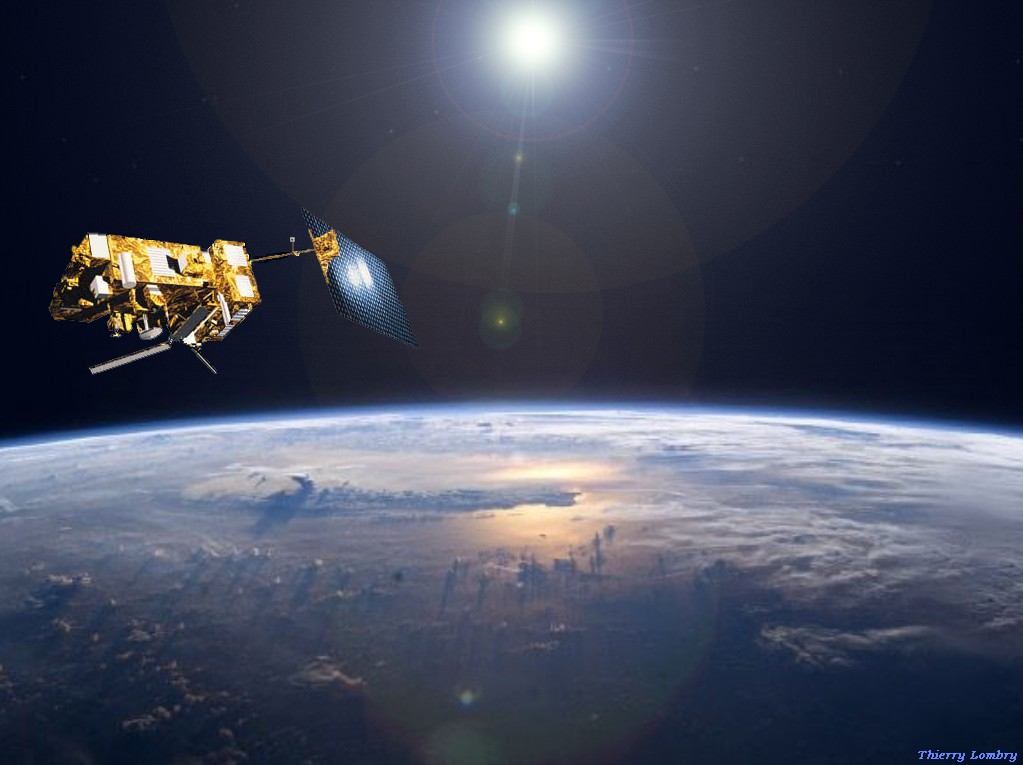
\includegraphics[height=\paperheight, keepaspectratio]{images/low_orbit}}%
\begin{frame}
\end{frame}
\begin{frame}
    \frametitle{About that circularizing}
    \begin{block}{}
        We are now almost in low earth orbit but still falling down. Our orbit could still cross the atmosphere.
        So we need to learn how to manipulate our orbit while in space.
    \end{block}
    \begin{block}{Basics}
        Movement on an orbit generally affects the opposite side of the orbit.
    \end{block}
\end{frame}
\begin{frame}
    \frametitle{Adjusting orbits}
    \begin{block}{}
        \begin{center}
            At any point on the orbit you can burn in 3 directions: up/down, left/right, forwards/backwards
        \end{center}
    \end{block}
    \begin{block}{}
        \begin{center}
            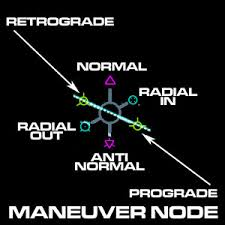
\includegraphics[scale=0.8]{images/maneuver_node}
        \end{center}
    \end{block}
\end{frame}
}

\begin{frame}
    \frametitle{Prograde}
    \begin{center}
        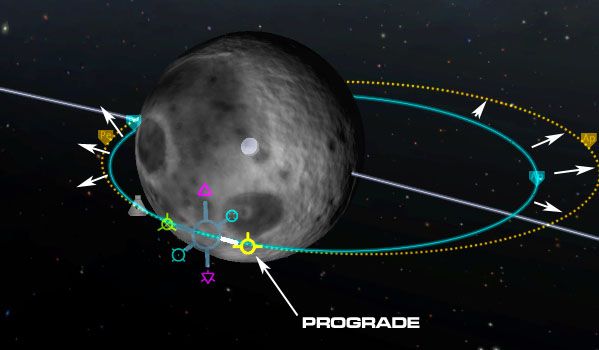
\includegraphics[scale=0.5]{images/prograde}
    \end{center}
\end{frame}
\begin{frame}
    \frametitle{Normal}
    \begin{center}
        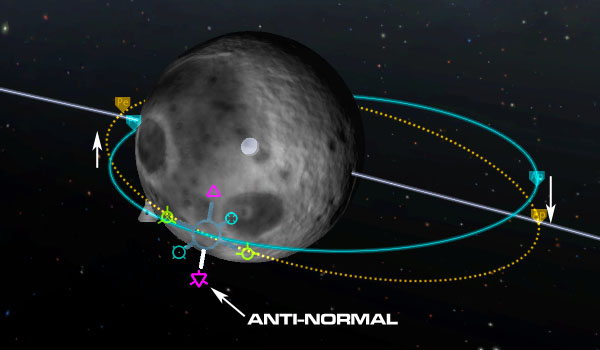
\includegraphics[scale=0.5]{images/anti_normal}
    \end{center}
\end{frame}
\begin{frame}
    \frametitle{Radial}
    \begin{center}
        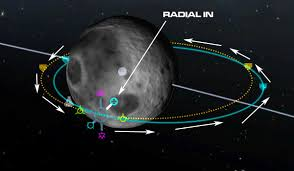
\includegraphics[]{images/radial}
    \end{center}
\end{frame}
